\documentclass[../report.tex]{subfiles}
\begin{document}


% Approach(es)
% Provide a brief review of prior work on this problem (at least 5 papers)
% Describe in detail about the approach(es) you use in this project
% Justify your algorithm choices through reasons and/or experiments

\section{Methodology}

\subsection{Reinforcement Learning Fundamentals \& Reversi}

\paragraph{Environment \& Markov Decision Processes (MDPs)}
An MDP is a network of states and actions that result in rewards. We denote all states $s\in S$, all actions $a\in A$, and all rewards as $r(s,a)\mapsto\mathbb{R}$ with . Additionally, each action has a probability of $P(s,a,s')$ of occuring. Finally, The states actions, rewards and probabilities are all set by the environment. In Reversi the state is represented by two parts: the board and the current player. The board consists of 64 grid spaces that can be each occupied by either a Black disk, a White disk, or no disk and can be represented via a 2D-matrix of \{-1,0,1\} respectively. An action in Reversi can be denoted by a pair ranging from (1,1) to (8,8) denoting the action of placing a disk. The resulting state of an action is one that flips all consecutive opponent disks in between the disk placed, and other surrounding disks. The reward is 0 for a loss, 0.5 for a draw and 1 for a win, with all other states being 0 reward. 

\paragraph{Policy}
The policy for a given state, denoted $\pi(s)$, produces an action dependent on the state for the environment. Many different policies exist with different methods for determining an action.

\paragraph{Agent}
An agent is an active participant in the environment, with which all reinforcement learning is centered on. That is, the agent progress through the an MDP of an environment with some given policy $\pi$. Each state $S_t$, action $A_t$, and reward $R_t$ are recorded by each time step $t$ to $T$ where $T$ is the terminal state.

\paragraph{Long-Term Reward}
For an Agent, the long-term reward of a given state is defined as the cumulative reward for all states in the environment at each time-step. That is, $G_t=R_t+G_{t+1}$.

\paragraph{Q-Function}
In an ideal setting, the Q-function, denoted $Q(s,a)$, measures the cumulative future reward of the current state-action pair, i.e., $G_t$. Thus, it reasons that the optimal policy that uses Q-learning is the policy,
\begin{equation}\label{eq:policy}
    \pi(s)=\arg\max\limits_{a}(Q(s,a))
\end{equation}

\paragraph{Value-Function}
In an ideal setting, the Value-function, denoted $V(s)$, measures the longperfectly estimates the best the cumulative future reward of the current state-action pair. Thus, it reasons that the optimal policy that uses Q-learning is the policy,

\paragraph{Reward-Shaping}
Additionally, in environments with sparse rewards, it may be necessary to introduce an additional hand-crafted reward to the current reward. If the reward from one state following an action to another is given by $R(s,a,s')$ then a shaped reward will be given by, $R'(s,a,s') = R'(s,a,s') + F(s,a,s')$ following some shaping function $F$.  


\subsection{Q-Approximation}\label{sec:q-approx}
Q-Learning is a model-free approach to reinforcement learning by learning a policy through an estimated Q-function. Using a combination of the current state and action, Q-Learning attempts to approximate the cumulative future reward of the current state-action pair and update itself accordingly. To do so, we use the Bellman equation,
\begin{equation}\label{eq:bellman_update}
    Q(s,a) \leftarrow Q(s,a) + \alpha [ r(s,a) + \gamma \max_a Q(s',a) - Q(s,a)]
\end{equation}
Where $\alpha$ is the step-size or learning rate hyperparameter and $\gamma$ is the hyperparameter discerning the discount factor, or more simply, the importance of long-term reward

As for policy selection, the $\epsilon$-greedy policy is used which has the benefits of exploring possible states, and also determining the effectiveness of the current $Q(s,a)$ values. That is, choosing some policy based on,
\begin{equation}\label{eq:epsilon-greedy}
    \pi_\epsilon(s)=
    \begin{cases}
        a \sim Unif(A)      & \text{with probability}\, \epsilon \\ 
        \arg\max\limits_{a}(Q(s,a))         & \text{with probability} \, 1-\epsilon
    \end{cases}
\end{equation}
Where $\epsilon\in[0,1]$.

\paragraph{Deep Q-Learning \& Neural Networks}
We note that Q-learning is often performed using a Q-table of some sort. However, for large state-action spaces this quickly becomes infeasible for the reason finite storage capacity. As a work around, Neural Networks can be used in lieu of this restriction as an abstraction of the Q-table in exchange for a more complex learning algorithm.

\begin{figure}
    \centering
    \begin{minipage}{0.35\textwidth}\label{fig:nn535}
        \centering
        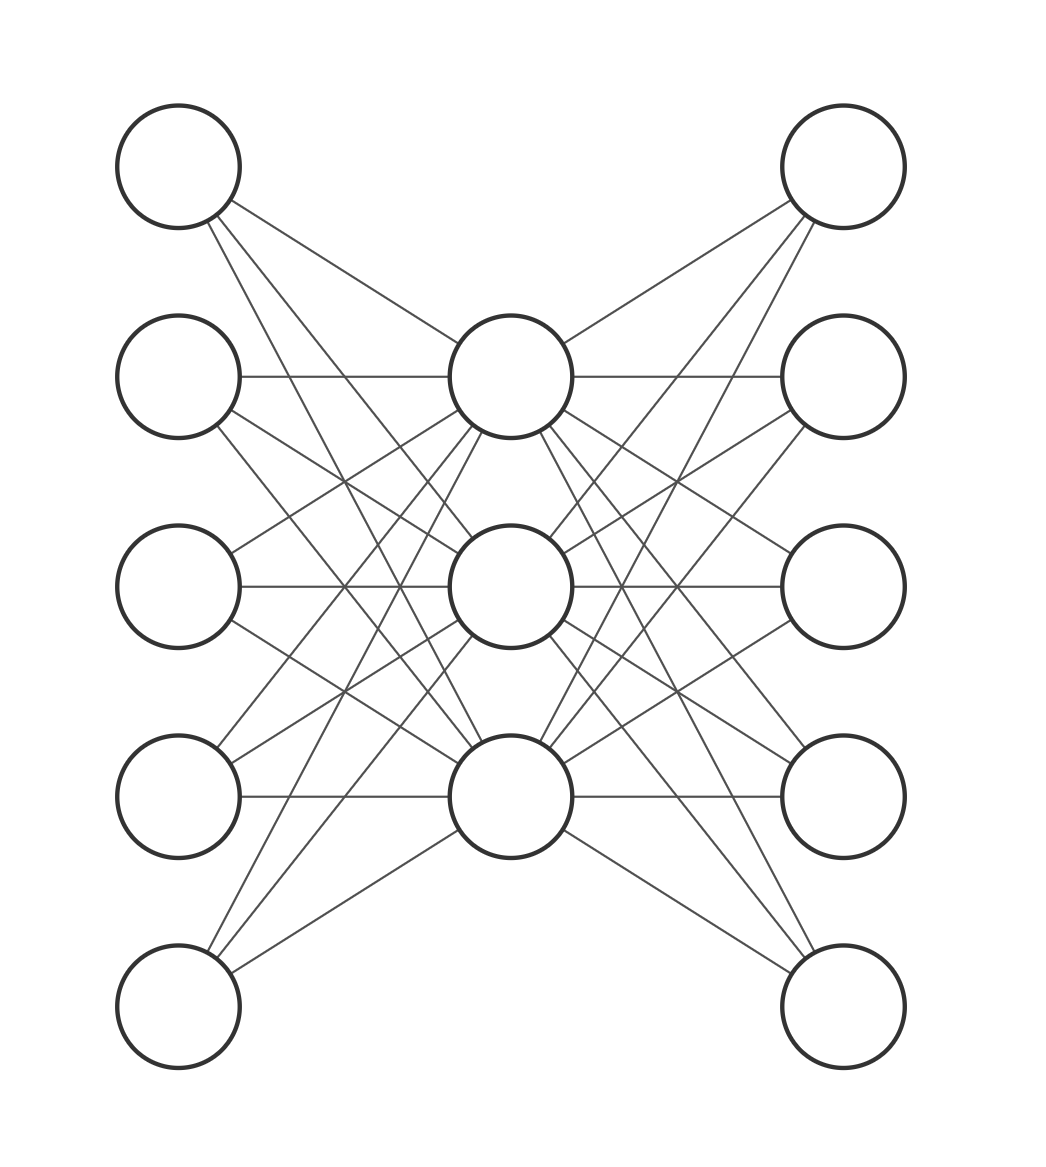
\includegraphics[width=0.9\textwidth]{nn535.png}
        \caption{An environment with 5 states and 5 actions with a DQN that maps $S \mapsto Q(s,a) \times A$ }
    \end{minipage}\hfill
    \begin{minipage}{0.35\textwidth}\label{fig:nn531}
        \centering
        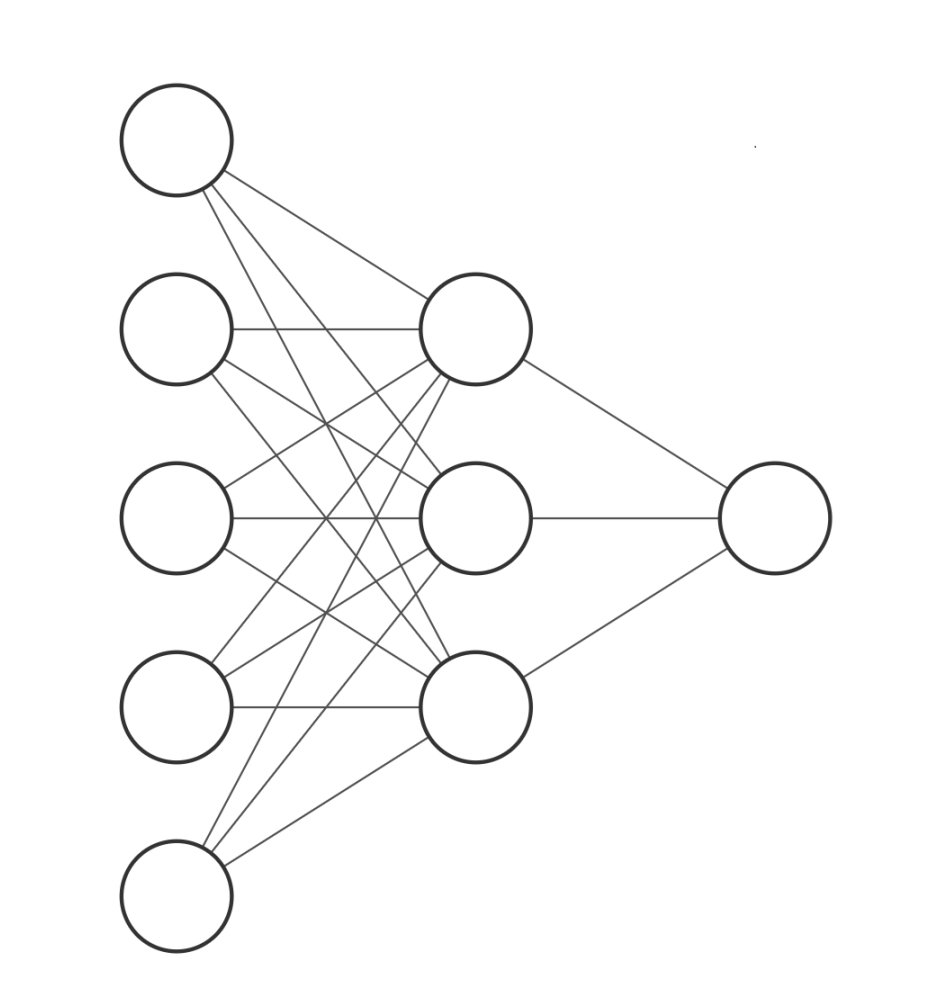
\includegraphics[width=0.9\textwidth]{nn531.png}
        \caption{An environment with 3 states and 2 actions with a DQN that maps $S\times A \mapsto Q(s,a)$ }
    \end{minipage}
\end{figure}

Literature on Deep Q-learning have been shown to implement this in several ways. Notably, for discrete action spaces, it is common such as in \cite{ree13} to use a neural network with simply a state as input, and all resulting Q-values for that state and all possible actions (\ref{fig:nn535}). Others use a neural network with a state-action pair as input, and only the resulting Q-values for output \ref{fig:nn531} as seen in \cite{ank13}. 


\subsection{Deep Q-Learning and Reversi/Othello}
We aim to implement Deep Q-learning within the game space using several methods. Firstly, we intend to use both types of neural networks described in section \ref{sec:q-approx}. With Q-learning being an off-policy learning approach, we are able to use an experience replay buffer such that past state-action pairs and their resulting state and rewards can be used as another way to train the agent. We further intend to use self-play, a method that uses a previous version of the current model being trained as the opponent policy. Finally, we also intend to explore the feasiblity of using reward shaping.

\paragraph{Experience Replay}
A benefit of off-policy learning is the ability to learn from past actions just as well as current ones, thus storing past experiences are beneficial. Inspired by \citet{mnih2013playing}, we store an experience replay buffer with $(s,a,r,s')$ after each action of the agent. Where $s'$ is the resulting state of performing $a$ at $s$ and the opponent takes their turn. We can then train the agent with the experience replay buffer.

\paragraph{Self-Play}
With self-play, an agent will play against the same, but earlier iteration of the current model one during training, which has been shown, such as in \citet{ree13} which has been shown to be beneficial. Specifically, we will use the 5th previous iteration of the current model as to introduce some randomness to learning

\paragraph{Reward Shaping}
While complex reward shaping exists such as in \cite{ng1999policy}, this requires extensive expert knowledge of the environment as this is a tangible guideline for the agent to follow. Instead, we opt for a simpler reward shaping algorithm,
\begin{equation}\label{eq:simple-reward-shaping}
    F(s,a,s') = \frac{(\text{\# Of Disks Of Current Agent's Color})}{64}
\end{equation}

\paragraph{Neural Network}
We will implement two networks with the following characteristics,
\begin{itemize}
    \item Network 1: An input of size 67 consisting of a combination of a state $s$ and action $a$ ($64$ grid-squares $+ 1$ current player $+ 2$ values for grid location of the next action). An output consisting of size 1, a proxy for $Q(s,a)$.
    \item Network 2: An input of size 65 representing a state $s$ ($64$ grid-squares $+ 1$ current player). An output consisting of size 64, a proxy for $Q(s,a)\:\forall a \in A$ given that there are 64 actions ( (1,1) to (8,8) ) regardless of legality.
\end{itemize}
Each network will have 3 hidden layers each of size 64. All nodes will use sigmoid activation function, and a loss of MSE will be used for computation of back propogation. Network values are fitted against the updated $Q(s,a)$ values. That is, the model is fitted against,
\begin{equation} \label{eq:nn-q-update}
    Q(s,a) = r(s,a) + \gamma \max_a Q(s',a)
\end{equation}
In regards to network 2, the update is carried out the same, with the additional requirement that the update is a size 64 array of 0's where corresponding action $a$ in the original $Q(s,a)$ is set to the value of (\ref{eq:nn-q-update}). Both networks will be fitted after a round has been played with the entirety of the replay buffer, which includes the round that had just been played.

The hyperparameters used for all models was,
\begin{itemize}
    \item $\alpha=0.001$
    \item $\gamma=0.1$
    \item $\epsilon=0.2$ Decaying linearly to $\epsilon=0$ at the final episode
    \item A replay buffer of size 4096
    \item Iteration of learning until no significant improvement in learning has occured for 10 episodes.
\end{itemize}

\paragraph{Experiments}
We aim to find out the optimal Deep Q-network through a set of experiments. That is, we wish to find the highest performing network that has generalized the best. In both \citet{ree13} and \citet{VANECK20081999}, a dueling like structure was used to test all networks involved. We similarily follow this approach and extend it to a tournament structure. That is, we first find the highest performing networks against a random policy opponent, and then rank them each against one another.
\end{document}